%!TEX root = ../dissertation.tex
\chapter{Analisi dei dati}
\label{AnalisiDeiDati}
Ora che è presente un database popolato di tutti i metadati necessari per ricercare i file raw di interesse, il prossimo passo è leggere ed estrarre correttamente i dati dai file.

Il sistema utilizza inoltre le librerie esterne matplotlib e plotly per produrre grafici, grafici di dispersione 2D e 3D, e istogrammi, allo scopo di visualizzare e studiare i dati estratti.

\section{Archiettura generale}

Il sistema di analisi dei dati può essere diviso in due parti principali:

\begin{itemize}
	\item la lettura dei dati dai file raw e dal database. Per questo scopo la classe BinaryReader si occupa della lettura corretta dei file raw (chiamati anche file binari), mentre la classe DataFetcher utilizza BinaryReader e uno dei client di comunicazione con il database visti nella sezione \ref{DiagrammaDelleClassiDMD} per raccogliere i dati di interesse e prepararli alla visualizzazione.
	\item la visualizzazione dei dati attraverso grafici con la classe DataPlotter che comprende la creazione dei grafici più significativi e l'interazione con i grafici stessi
\end{itemize}

\begin{figure}
	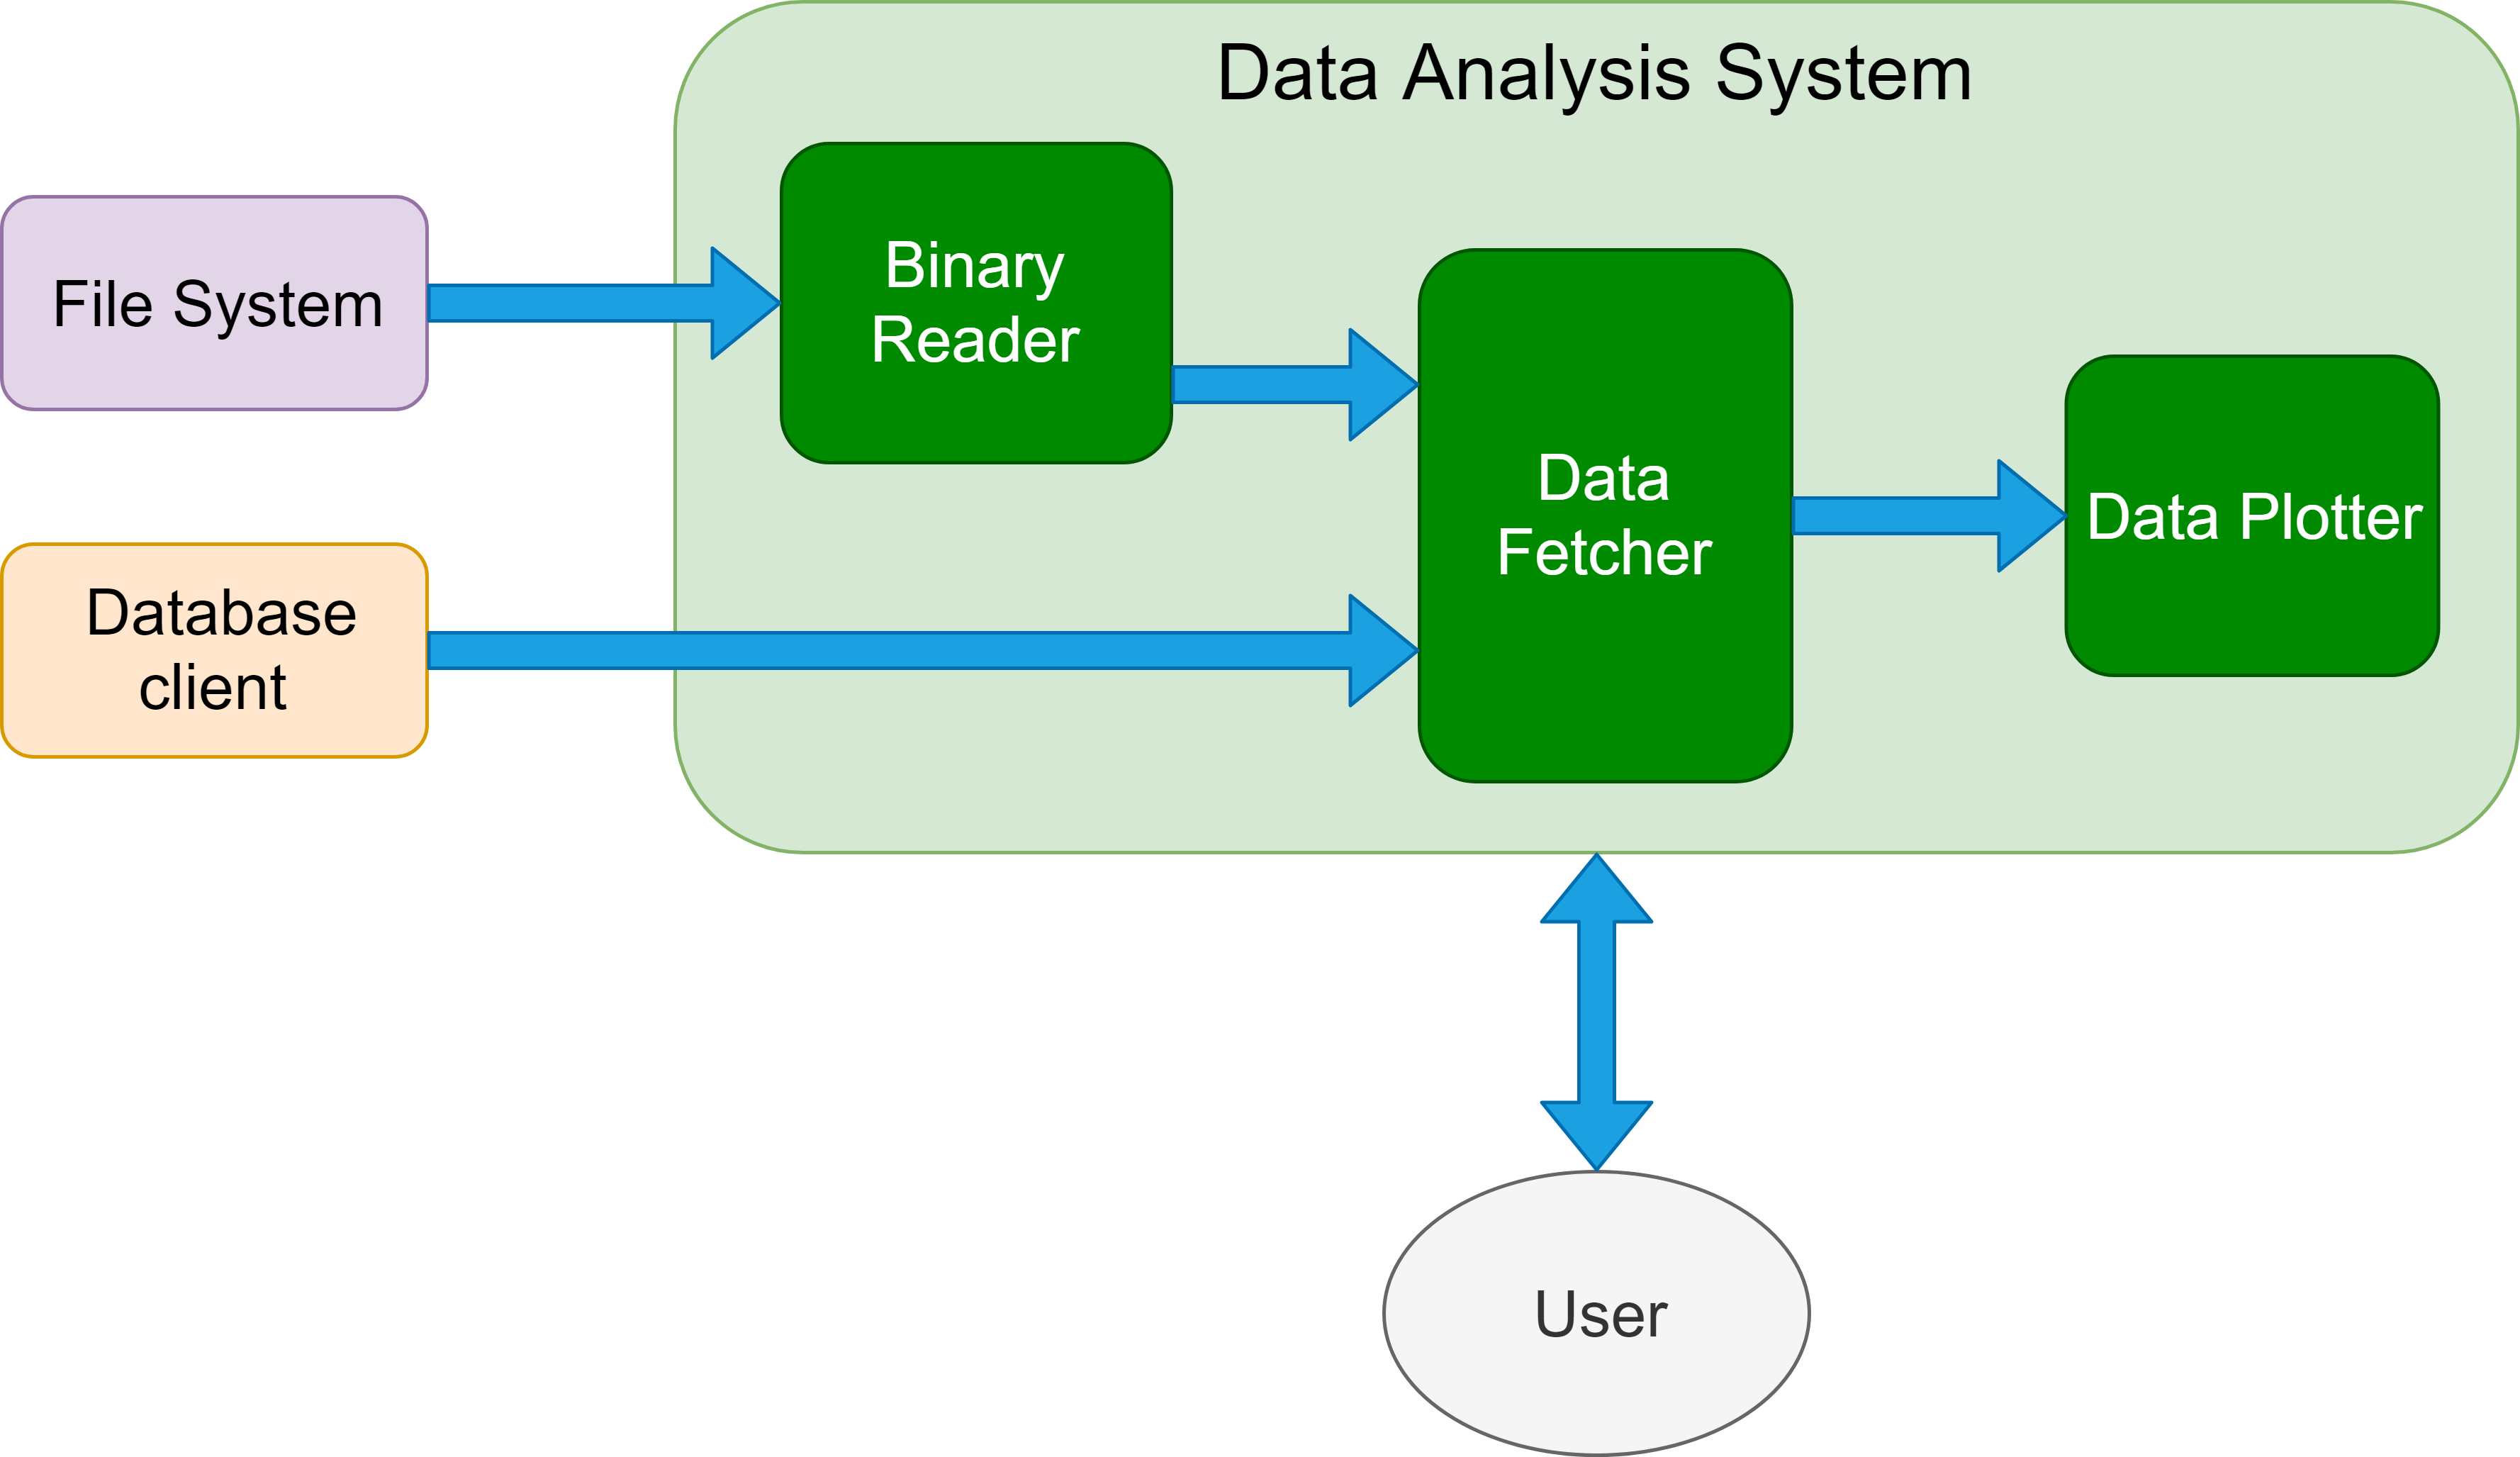
\includegraphics[width=\textwidth]{figures/ArchitetturaDA}
	\caption[Architettura del sistema di analisi dei dati]{ Architettura generale del sistema di analisi dei dati  e le interazioni verso le componenti esterne al sistema stesso.
		\label{fig:ArchitetturaDA}}
\end{figure}


\section{Lettura e contenuto dei file raw}
I file sono creati attraverso LabVIEW, un programma della National Instruments che si occupa di gestire la lettura dei sensori, e non sono pensati per essere aperti con programmi esterni. Per questo motivo la lettura dei file raw diventa complessa attraverso solo l'uso di Python.

I file raw sono dei file binari che posso essere in uno dei formati proprietari BIN o BIX. Il formato influisce la struttura del file e come sono stati salvati i dati al suo interno.

Il contenuto dei file cambia inoltre in base alla configurazione del Multiphase Flow Meter, di conseguenza ogni BIN e BIX possono essere di tipi diversi, distinti dal campo "BIN type" o "BIX type" all'interno del file.

Ogni file raw contiene un insieme di variabili determinato dal formato e dal tipo del file stesso. Ogni variabile è caratterizzata da:
\begin{itemize}
	\item \texttt{type}: rappresenta il tipo della variabile, ad esempio Int32, UInt32, Float, Boolean.
	\item \texttt{batch size}: rappresenta il numero di letture che vengono effettuate al secondo per quella variabile, può variare da 1 a 2500.
	\item \texttt{data}: un array che contiene le letture effettive del sensore
\end{itemize}

I dati contenuti in queste variabili corrispondo alle letture dei sensori presenti nel Multiphase Flow Meter al momento del test.

\section{Grafici e analisi dei dati}

L'analisi dei dati comincia dalla scelta una delle cartelle dei test presenti nel server aziendale, si ricorda che ogni test rappresenta una serie di letture effettuate in ambiente controllato in un laboratorio. Scelto uno specifico test è possibile creare un grafico di dispersione in base alle proprietà GVF e WLR (descritte nella sezione \ref{"StrutturaDeiDati"}) di tutti i file raw presenti in quella cartella di test. Questa operazione sfrutta le informazioni salvate nel database creato in precedenza in modo da non dover esplorare di nuovo tutta la cartella.
Si ottiene quindi un grafico simile a quello in figura \ref{fig:GVFWLRscatter} dove ogni punto rappresenta un file raw ed è posizionato in base alle proprietà GVF e WLR che aveva il flusso nel momento in cui è stata effettuata la lettura. Si può notare che i punti sono per la maggior parte allineati in una struttura a matrice, questo perché le proprietà del flusso sono variate in modo controllato per coprire più casi possibili. 

\begin{figure}[H]
	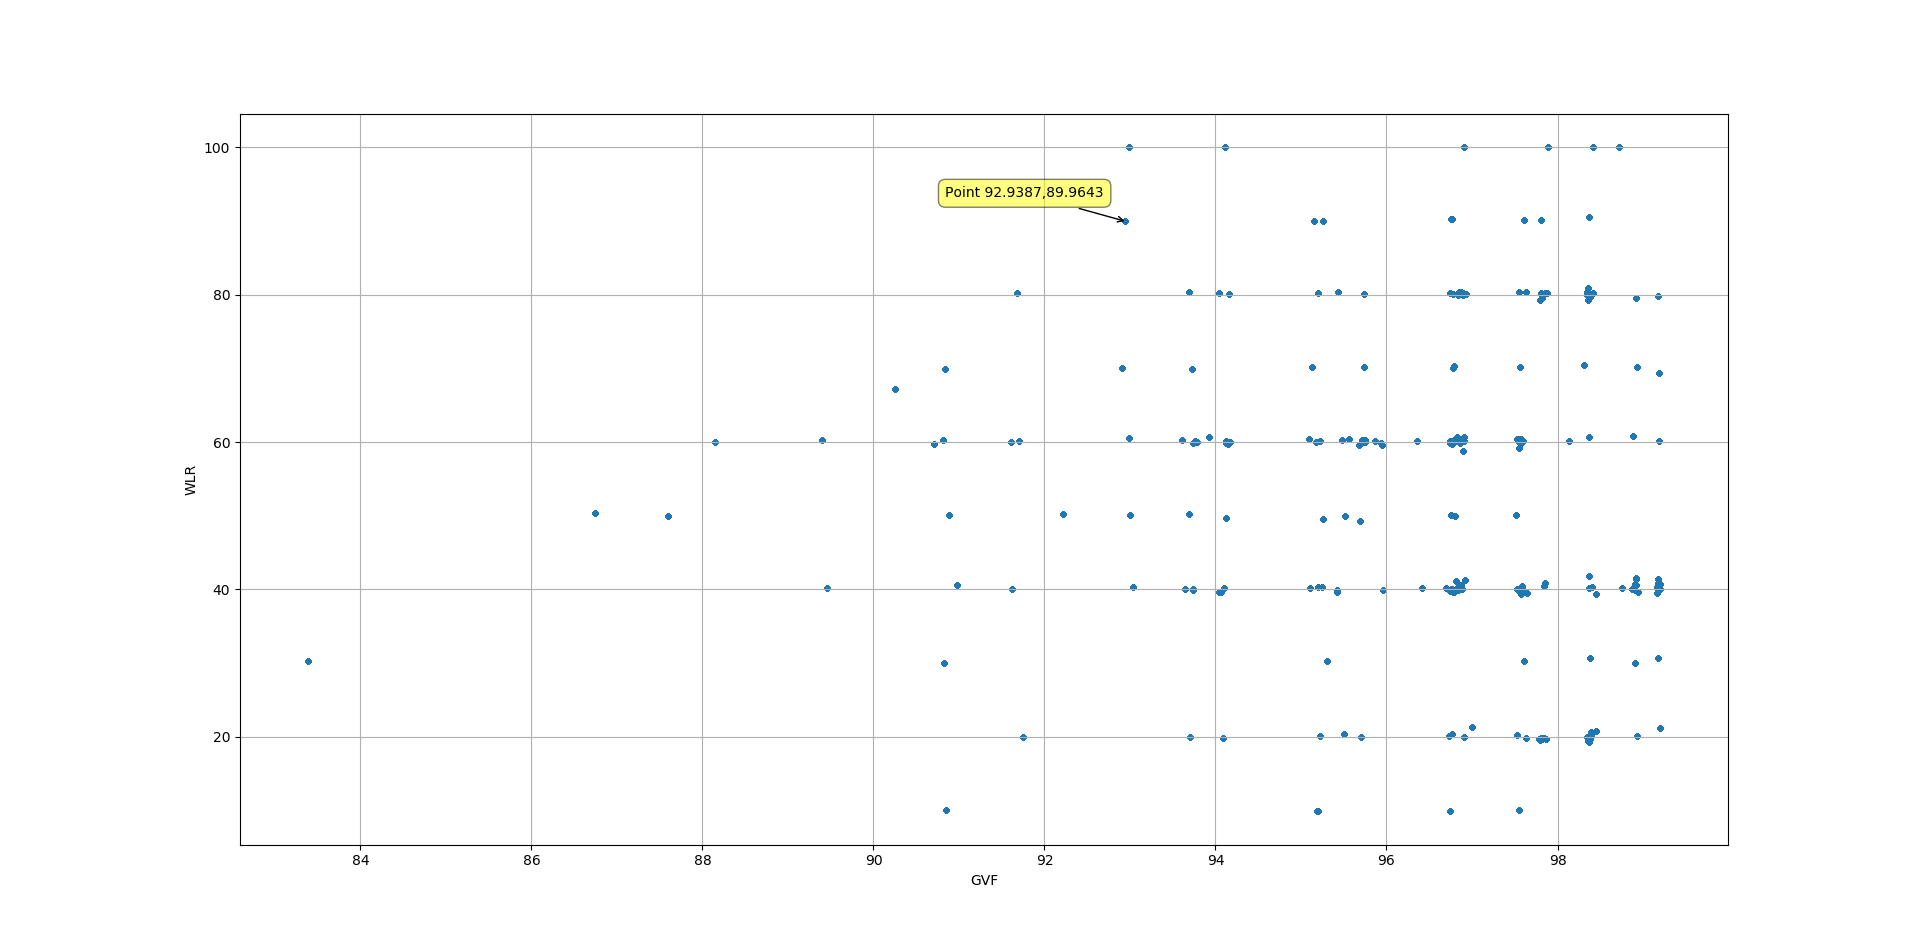
\includegraphics[width=\textwidth]{figures/GVFWLRscatter}
	\caption[Grafico di dispersione GVF-WLR]{ Grafico di dispersione tra le variabili GVF e WLR,  ogni punto rappresenta un file raw ed è posizionato in base alle proprietà GVF e WLR che aveva il flusso nel momento in cui è stata effettuata la lettura. 
		\label{fig:GVFWLRscatter}}
\end{figure}

Cliccando un punto all'interno di questo grafico è possibile vedere graficamente i valori di tutte le variabili del file raw associato a quel punto (figura \ref{fig:MatrixPlot}). Per motivi di velocità e dimensione i grafici delle variabili sono approssimati e contengono solo il massimo in verde, la media in arancione e il minimo in blu di ogni secondo di lettura.

\begin{figure}[H]
	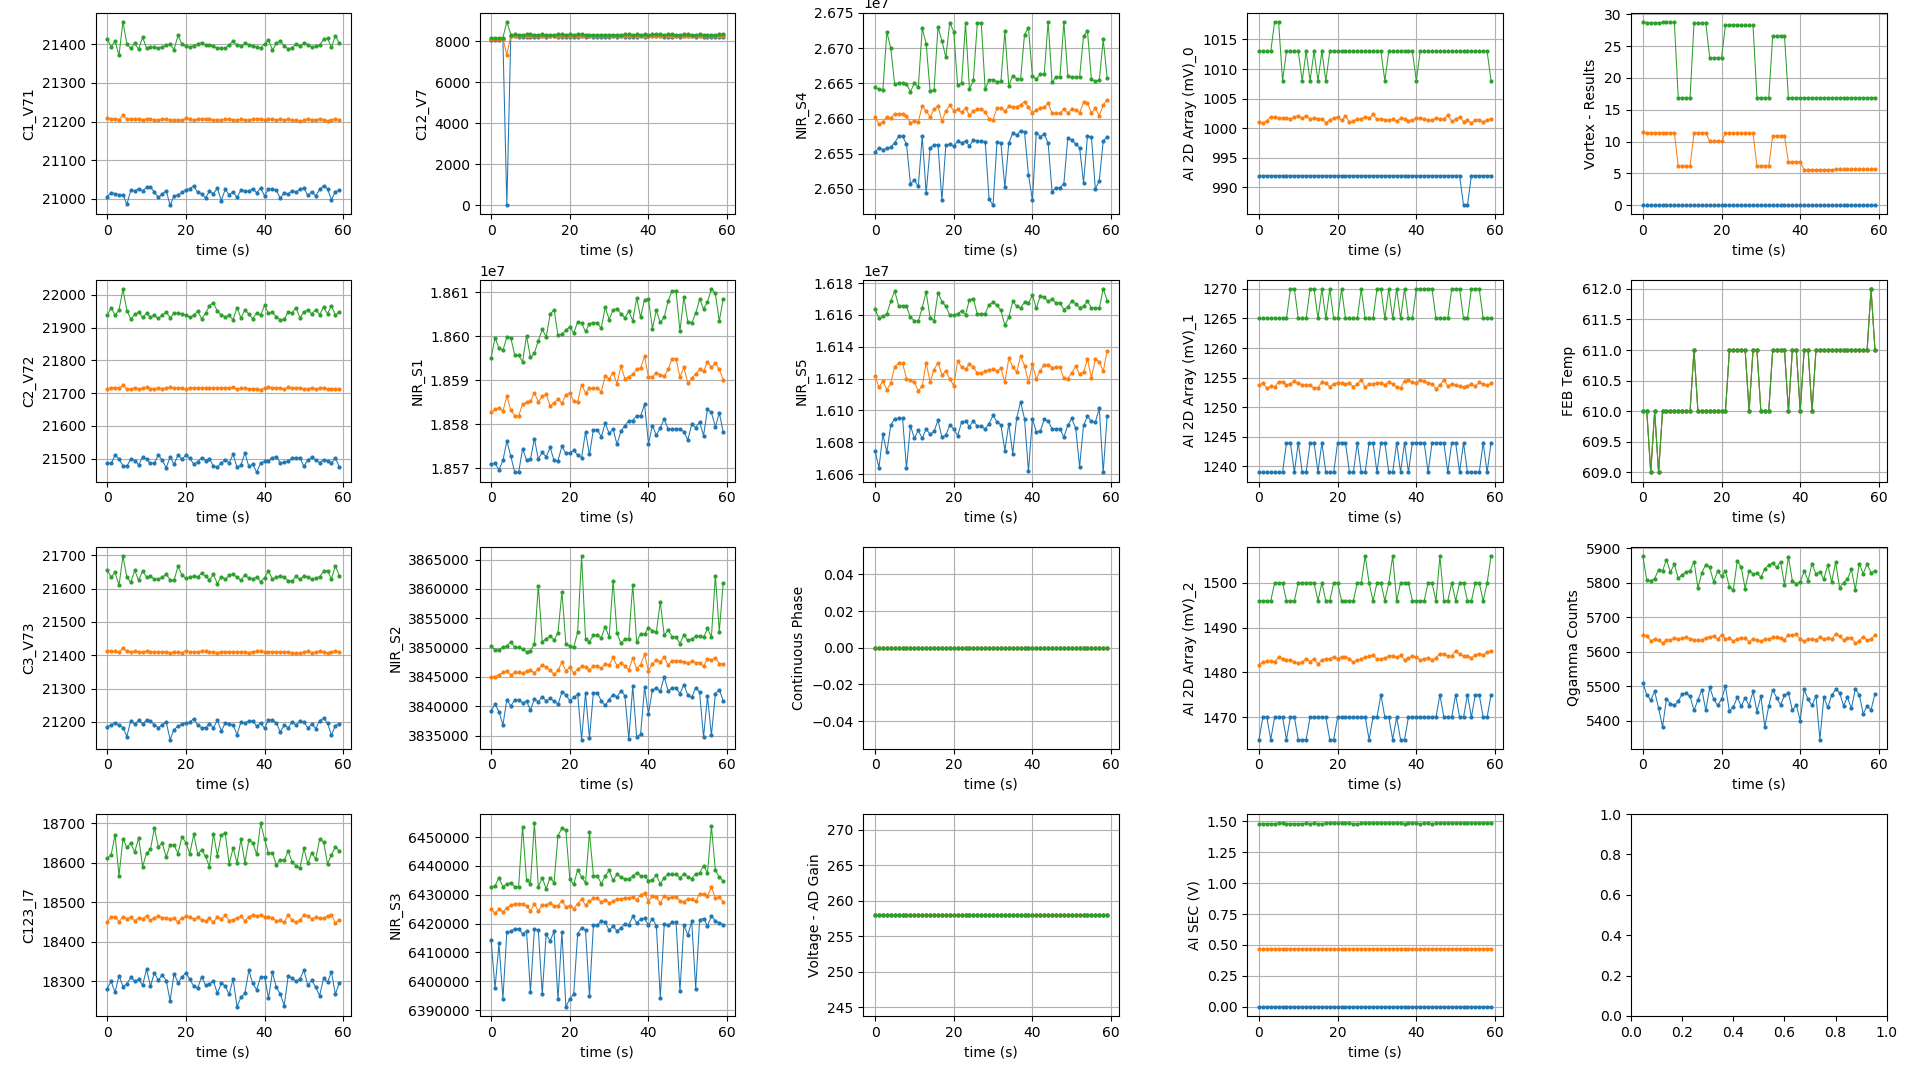
\includegraphics[width=\textwidth]{figures/MatrixPlot}
	\caption[Grafici delle variabili di un file raw]{ Grafici delle variabili di un file raw. La linea in verde indica i massimi di ogni secondo di lettura, in arancione le medie, in blu i minimi.
		\label{fig:MatrixPlot}}
\end{figure}

I grafici delle variabili sono selezionabili tenendo premuto il tasto shift o ctrl della tastiera e cliccando da uno a tre grafici. A seconda del numero di grafici selezionati viene mostrato una tipologia di grafico diversa.

Selezionando un solo grafico si visualizza un nuovo grafico contenente tutti i punti di quella specifica variabile, e non solo un'approssimazione. Allineato al grafico dei punti è presente un istogramma orizzontale che mostra più chiaramente quali sono i valori più frequenti per quella variabile.

\begin{figure}[H]
	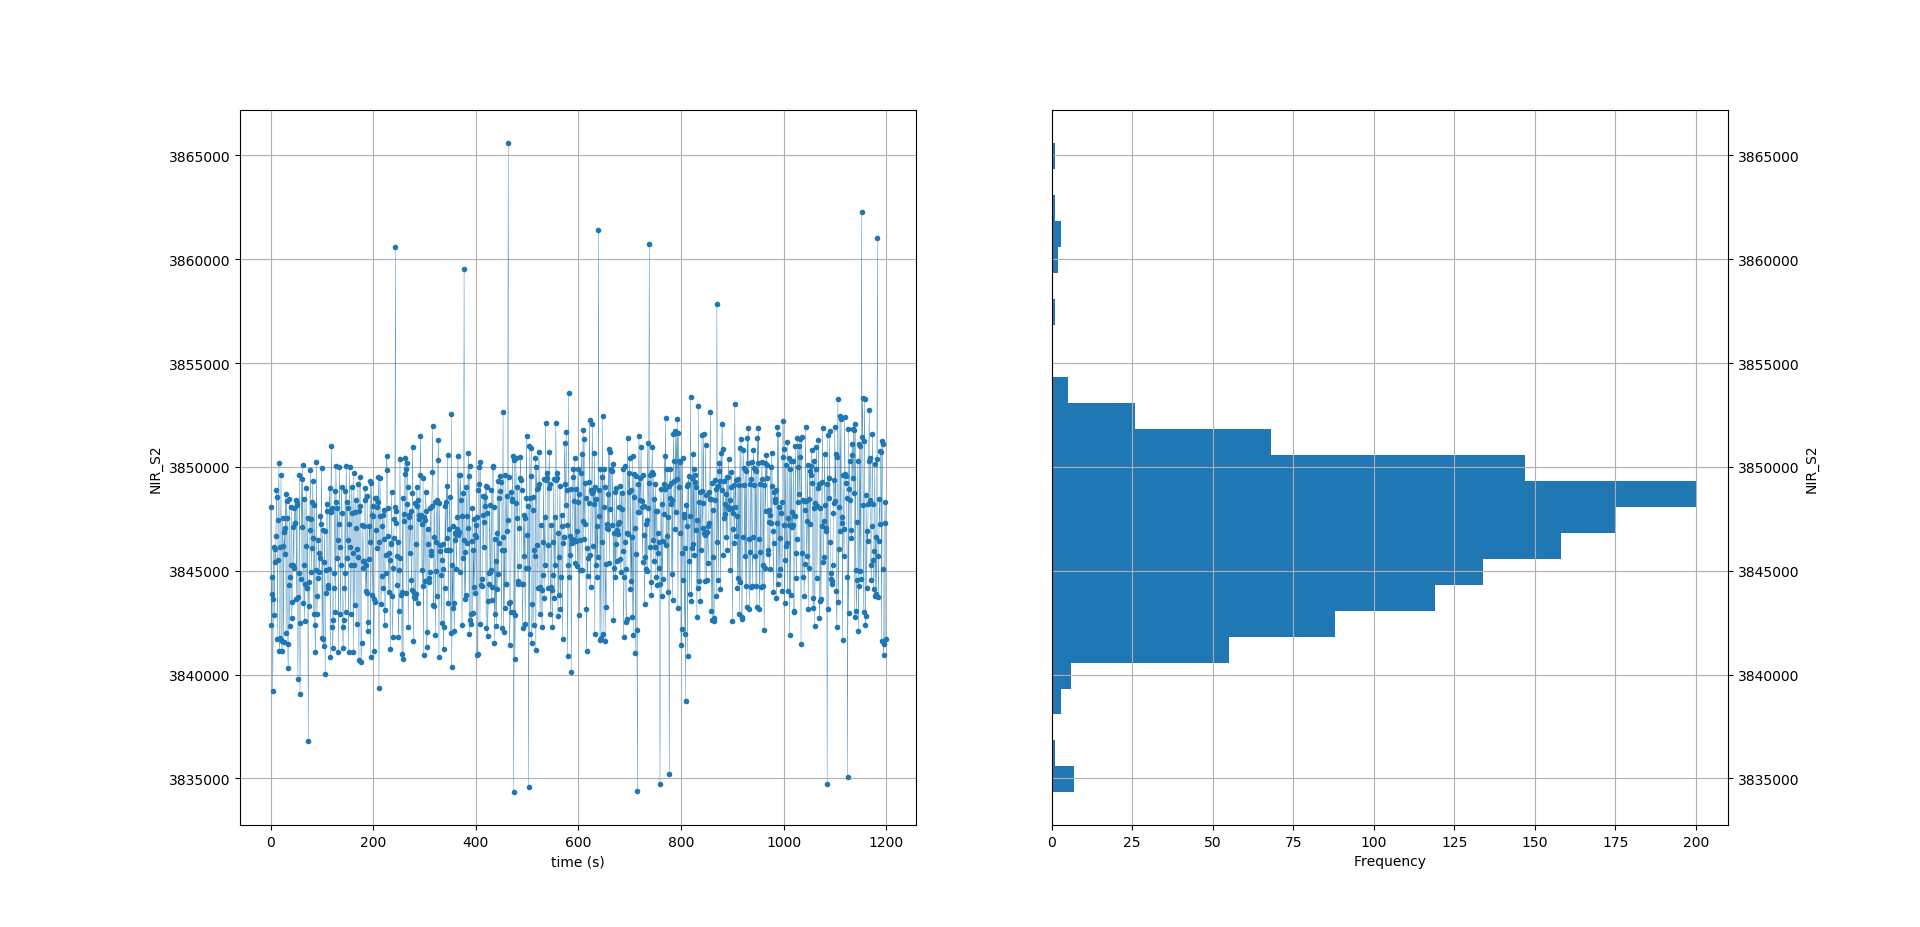
\includegraphics[width=\textwidth]{figures/SimplePlotHistogram}
	\caption[Grafico e istogramma di una variabile]{ Grafico e istogramma di una variabile. L'istogramma rappresenta i valori più frequenti.
		\label{fig:SimplePlotHistogram}}
\end{figure}


Selezionando due grafici si visualizza un grafico di dispersione delle due rispettive variabili. Questo grafico può essere utile per controllare se due variabili sono correlate, punti fuori dalla distribuzione potrebbero indicare delle anomalie. Due variabili correlate si riconoscono dalla posizione dei punti nel grafico stesso, se si dispongono lungo una o più linee diagonali sono correlate, se si dispongono in uno o più gruppi sparsi non sono correlate.

\begin{figure}[H]
	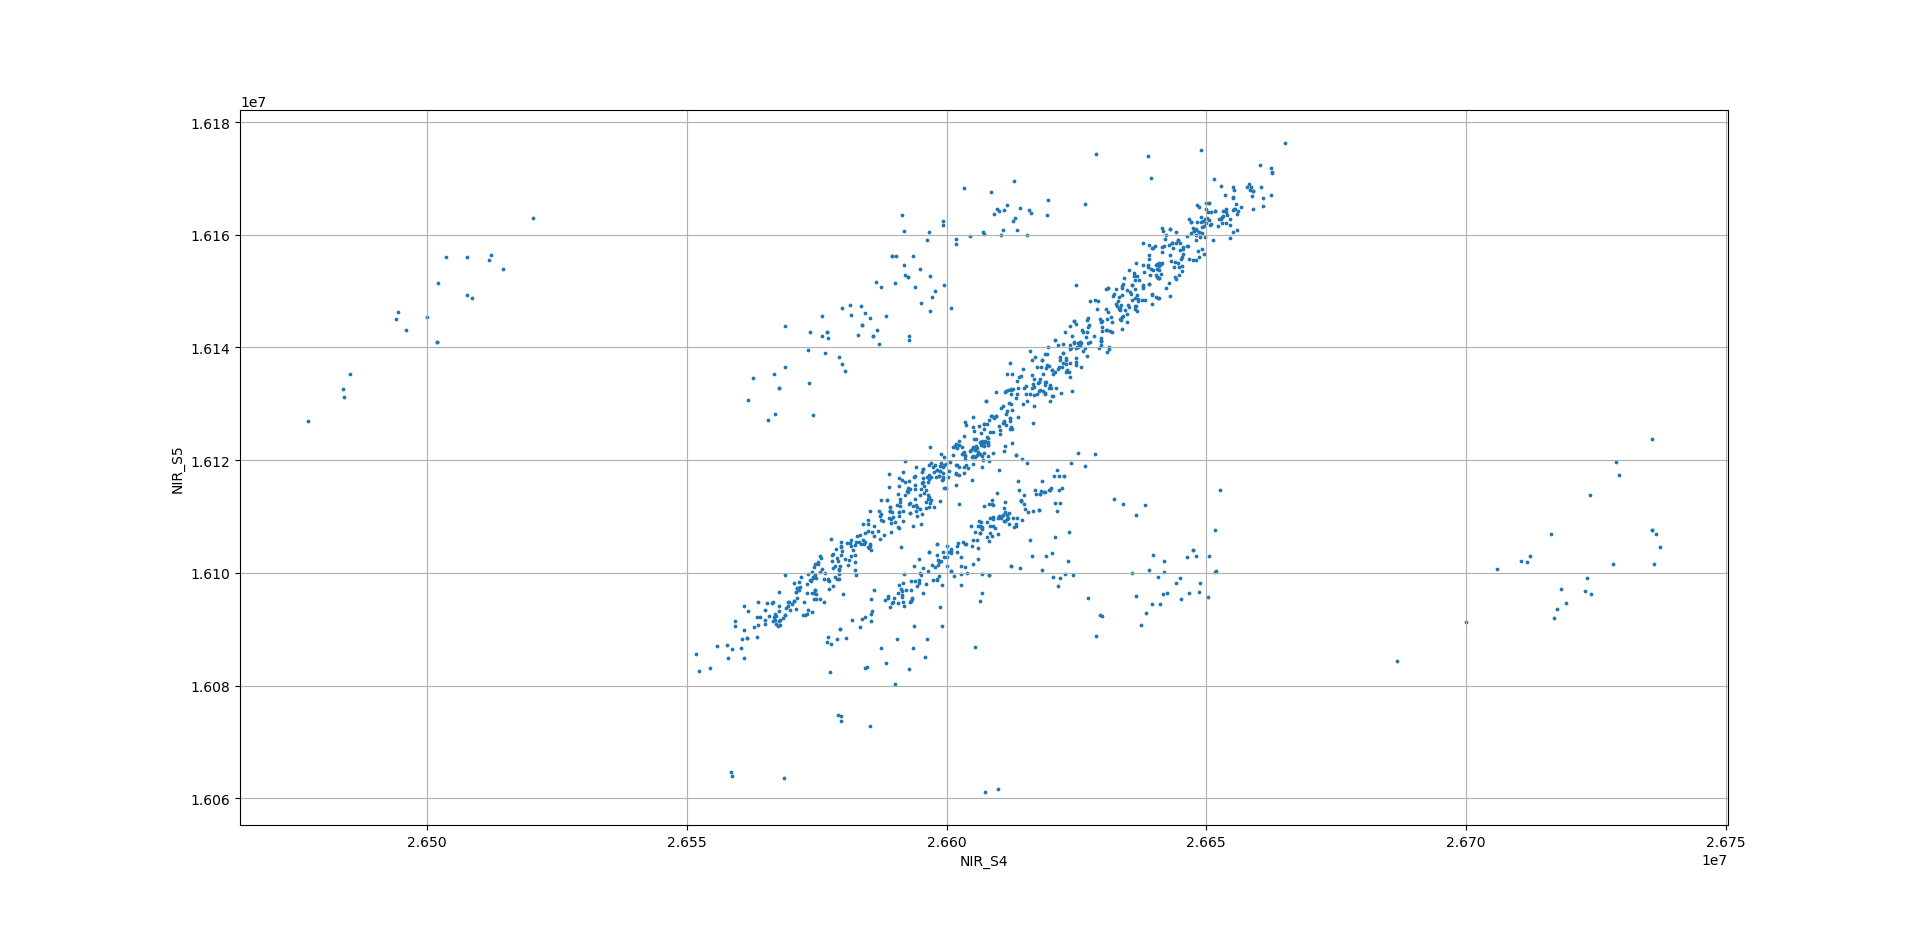
\includegraphics[width=\textwidth]{figures/2Dscatter}
	\caption[Grafico di dispersione di due variabili]{ Grafico di dispersione di due variabili. In questo caso sono si può notare che sono correlate.
		\label{fig:2Dscatter}}
\end{figure}

Selezionando tre grafici si visualizza un grafico di dispersione in 3D delle tre variabili selezionate, che si può spostare e ruotare a piacimento. Questo grafico è particolarmente utile quando si utilizzano tre variabili correlate tra di loro.

\begin{figure}[H]
	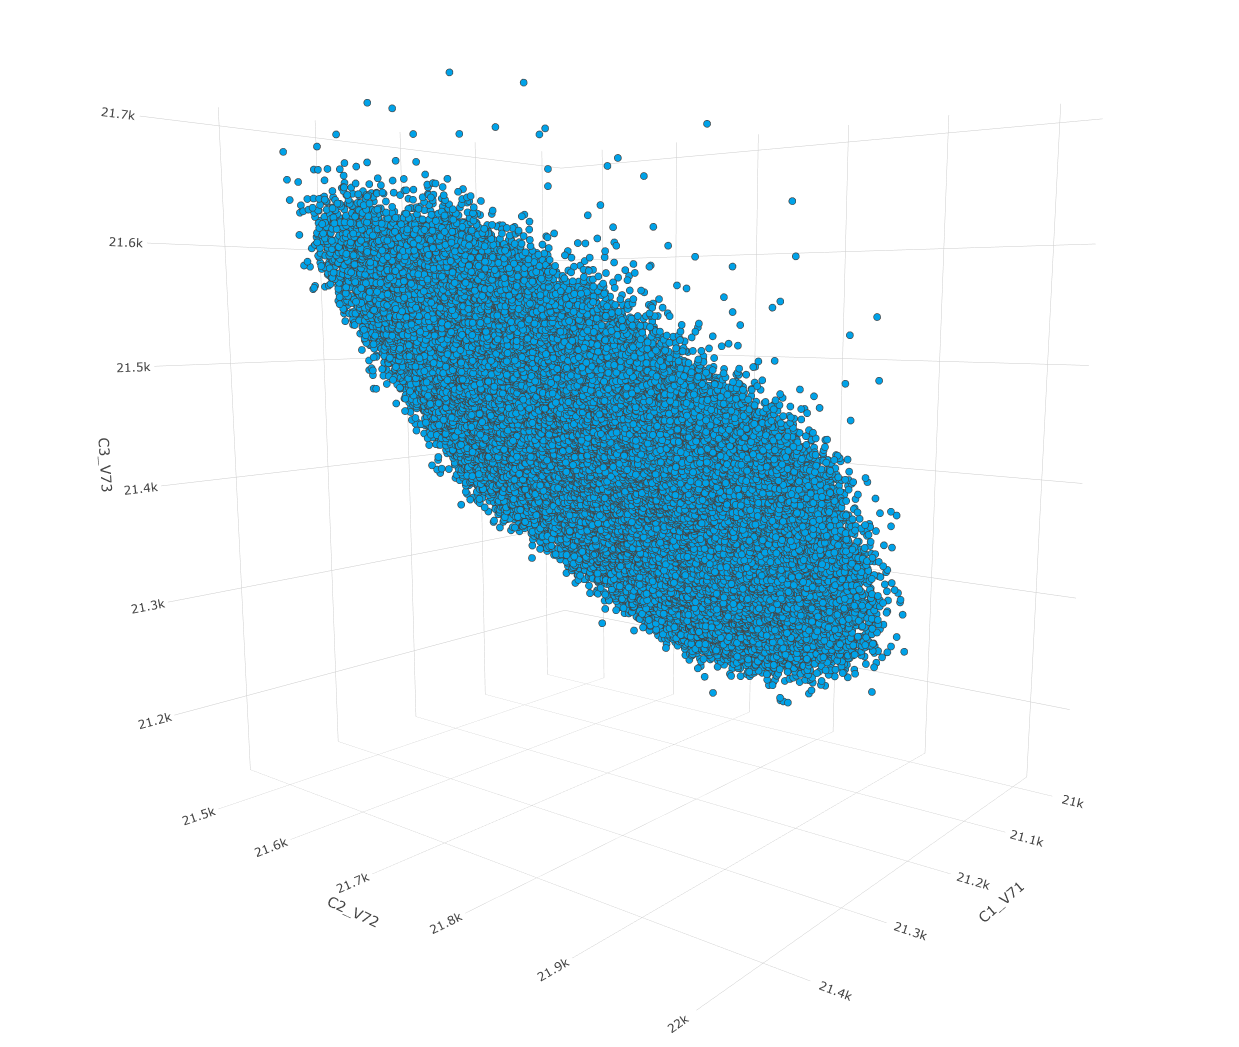
\includegraphics[width=\textwidth]{figures/3Dscatter}
	\caption[Grafico di dispersione di tre variabili]{ Grafico di dispersione di tre variabili. In questo caso i punti sono disposti a forma di disco perché le variabili C1\_V71 e C3\_V73 sono correlate tra loro ma non a C2\_V72.
		\label{fig:3Dscatter}}
\end{figure}

Ogni tipologia di grafico può essere visualizzata usando la libreria Matplotlib oppure Plotly in base a se si sono selezionai i grafici con shift o con ctrl. Si è lasciata la scelta perché entrambe le librerie hanno dei vantaggi e degli svantaggi a seconda del grafico che si vuole ottenere.

Matplotlib è molto veloce nella creazione del grafico ma con molti punti, intorno alle decine di migliaia, rallenta quando si prova a ingrandire, ruotare e selezionare una parte specifica del grafico.
Plotly impiega un paio di minuti per la creazione del grafico perché genera una pagina HTML indipendente, ma la manipolazione del grafico risulta veloce anche nell'ordine delle centinaia di migliaia di punti. Inoltre, essendo i grafici file HTML veri e propri, possono essere salvati e visualizzati offline, mentre Matplotlib permette solo il salvataggio di un'immagine statica del grafico perdendo l'interattività.

